% arara: xelatex
\documentclass[12pt]{article}

% \usepackage{physics}

\usepackage{hyperref}
\hypersetup{
    colorlinks=true,
    linkcolor=blue,
    filecolor=magenta,      
    urlcolor=cyan,
    pdftitle={Overleaf Example},
    pdfpagemode=FullScreen,
    }

\usepackage{tikzducks}

\usepackage{tikz} % картинки в tikz
\usepackage{microtype} % свешивание пунктуации

\usepackage{array} % для столбцов фиксированной ширины

\usepackage{indentfirst} % отступ в первом параграфе

\usepackage{sectsty} % для центрирования названий частей
\allsectionsfont{\centering}

\usepackage{amsmath, amsfonts, amssymb} % куча стандартных математических плюшек

\usepackage{mathtools}
\usepackage{comment}

\usepackage[top=2cm, left=1.2cm, right=1.2cm, bottom=2cm]{geometry} % размер текста на странице

\usepackage{lastpage} % чтобы узнать номер последней страницы

\usepackage{enumitem} % дополнительные плюшки для списков
%  например \begin{enumerate}[resume] позволяет продолжить нумерацию в новом списке
\usepackage{caption}

\usepackage{url} % to use \url{link to web}


\newcommand{\smallduck}{\begin{tikzpicture}[scale=0.3]
    \duck[
        cape=black,
        hat=black,
        mask=black
    ]
    \end{tikzpicture}}

\usepackage{fancyhdr} % весёлые колонтитулы
\pagestyle{fancy}
\lhead{}
\chead{}
\rhead{Econometrics midterm, March 2025}
\lfoot{}
\cfoot{}
\rfoot{}

\renewcommand{\headrulewidth}{0.4pt}
\renewcommand{\footrulewidth}{0.4pt}

\usepackage{tcolorbox} % рамочки!

\usepackage{todonotes} % для вставки в документ заметок о том, что осталось сделать
% \todo{Здесь надо коэффициенты исправить}
% \missingfigure{Здесь будет Последний день Помпеи}
% \listoftodos - печатает все поставленные \todo'шки


% более красивые таблицы
\usepackage{booktabs}
% заповеди из докупентации:
% 1. Не используйте вертикальные линни
% 2. Не используйте двойные линии
% 3. Единицы измерения - в шапку таблицы
% 4. Не сокращайте .1 вместо 0.1
% 5. Повторяющееся значение повторяйте, а не говорите "то же"


\setcounter{MaxMatrixCols}{20}
% by crazy default pmatrix supports only 10 cols :)


\usepackage{fontspec}
\usepackage{libertine}
\usepackage{polyglossia}

\setmainlanguage{english}
\setotherlanguages{english}

% download "Linux Libertine" fonts:
% http://www.linuxlibertine.org/index.php?id=91&L=1
% \setmainfont{Linux Libertine O} % or Helvetica, Arial, Cambria
% why do we need \newfontfamily:
% http://tex.stackexchange.com/questions/91507/
% \newfontfamily{\cyrillicfonttt}{Linux Libertine O}

\AddEnumerateCounter{\asbuk}{\russian@alph}{щ} % для списков с русскими буквами
% \setlist[enumerate, 2]{label=\asbuk*),ref=\asbuk*}

%% эконометрические сокращения
\DeclareMathOperator{\rank}{rank}
\DeclareMathOperator{\Cov}{\mathbb{C}ov}
\DeclareMathOperator{\Corr}{\mathbb{C}orr}
\DeclareMathOperator{\Var}{\mathbb{V}ar}
\DeclareMathOperator{\pCorr}{\mathrm{pCorr}}
\DeclareMathOperator{\col}{col}
\DeclareMathOperator{\row}{row}
\DeclareMathOperator{\hCov}{\widehat{Cov}}
\DeclareMathOperator{\hVar}{\widehat{Var}}


\let\P\relax
\DeclareMathOperator{\P}{\mathbb{P}}

\DeclarePairedDelimiter{\abs}{\lvert}{\rvert}
\DeclarePairedDelimiter{\norm}{\lVert}{\rVert}

\let\H\relax
\DeclareMathOperator{\H}{\mathbb{H}}


\DeclareMathOperator{\E}{\mathbb{E}}
% \DeclareMathOperator{\tr}{trace}
\DeclareMathOperator{\card}{card}

\DeclareMathOperator{\Convex}{Convex}

\newcommand{\SSR}{SS^{\text{res}}}
\newcommand{\SSE}{SS^{\text{expl}}}
\newcommand{\SST}{SST}
\newcommand{\hb}{\hat\beta}
\newcommand{\hy}{\hat y}
\newcommand \cN{\mathcal{N}}
\newcommand \dN{\mathcal{N}}
\newcommand \dBin{\mathrm{Bin}}


\newcommand \RR{\mathbb{R}}
\newcommand \NN{\mathbb{N}}





\begin{document}

Short rules: one A4 cheatsheet is allowed, calculators are ok, offline, 120 minutes.

\begin{enumerate}
    \item Consider approximating a hedgehog using two geometric shapes: 
    a cone for the nose and a half-sphere for the rest of the body. 
    
    Using a large dataset you have estimated the diameter $\hat D = 200$ mm and the length of the nose $\hat h = 25$ mm 
    with $se(\hat D) = 1$ mm and $se(\hat h) = 5$ mm.
    The latter is higher since the hedgehog might bite. 
    The estimators $\hat D$ and $\hat h$ are uncorrelated.
    
    \begin{minipage}{\textwidth}
        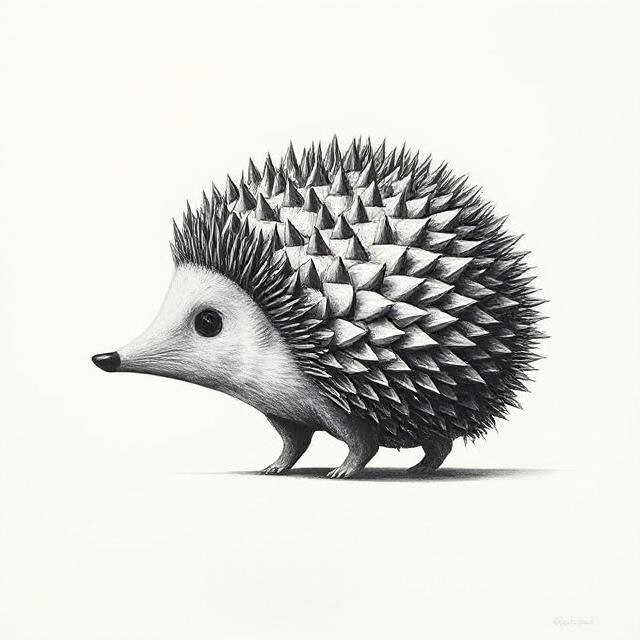
\includegraphics[scale=0.25]{hedgehog.jpg}
    \end{minipage}
    
    The sphere volume is $V_s = \pi D^3 / 6$. 
    The cone volume is $V_c = \pi D^2 h / 12$. 
    
    \begin{enumerate}
        \item {[5]} Find the standard error of the volume of the half-sphere hedgehog part using the delta method.
        \item {[5]} Find the standard error of the hedgehog volume using the delta method.
        % \item {[2]} Find the 95\% confidence interval for the hedgehog volume assuming asymptotic normality.
    \end{enumerate}
 
    \item The price level $p_t$ and production $q_t$ are endogeneous variables. 
    Taxes $a_t$ and income $b_t$ are exogeneous. 
    All variables are centered. 
    The structural form is given by the system
    \[
        \begin{cases}
            p_t = \alpha_1 q_t + \alpha_2 a_t + u_{1t} \\
            q_t = \beta_1 p_t + \beta_2 b_t + u_{2t}.
        \end{cases}        
    \]
    The estimates of the reduced form via equation-by-equation ols:
    \[
    \begin{cases}
        p_t = 2 a_t + 3 b_t \\
        q_t = - 3 a_t + 2 b_t.
    \end{cases}
    \]
    \begin{enumerate}
        \item {[6]} Recover the estimates of the coefficients in structural form.
        \item {[4]} Describe how you will estimate the standard errors of the structural form. 
    \end{enumerate}


    \item The price level $p_t$, production $q_t$ and interest rate $r_t$ are endogeneous variables. 
    Taxes $a_t$ and income $b_t$ are exogeneous. 
    All variables are centered. 
    The structural form is given by the system
    \[
        \begin{cases}
            p_t = \alpha_1 q_t + \alpha_2 a_t + u_{1t} \\
            q_t = \beta_1 p_t + \beta_2 b_t + u_{2t} \\
            r_t = \gamma_1 p_t + \gamma_2 q_t + \gamma_3 b_t + u_{3t} \\
        \end{cases}        
    \]
    \begin{enumerate}
        \item {[5]} Check the order condition for each equation. 
        \item {[5]} Check the rank condition for each equation.
    \end{enumerate}
    
    \newpage
    \item The probit model was estimated:
    $\hat\P(y_1 = 1 \mid x_i, d_i) = F(-0.3 + 0.2 x_i + 0.1 d_i)$.
    \begin{enumerate}
        \item {[3]} Forecast the odds of $y_1 = 1$ for $x_i = 1$, $d_i = 1$.
        \item {[3]} Find the partial effect of changing the value of the dummy variable $d_i$ from zero to one for $x_i = 1$.
        \item {[4]} Find the marginal effect of changing the value of the variable $x_i$ for $x_i = 1$ and $d_i = 1$.
    \end{enumerate}

    Hint: $\P(W \leq 0.1) = 0.54$ for a standard normal $W \sim \cN(0; 1)$.

    \item The probit model was estimated using $1000$ observations. 
    Standard errors are given in brackets.
    \[
    \hat\P(y_1 = 1 \mid x_i, d_i) = F(\underset{(0.01)}{-0.3} + \underset{(0.02)}{0.2} x_i + \underset{(0.01)}{0.1} d_i), \quad AIC = 606.
    \]
    \begin{enumerate}
        \item {[3]} Provide a 95\% confidence interval for $\beta_x$.
        \item {[4]} Find the log-likelihood of the trivial probit model, $\hat\P(y_1 = 1 \mid x_i, d_i) = F(\hb_0)$.
        \item {[3]} Compare the initial model and the trivial model using likelihood ratio test at 5\% significance level.
    \end{enumerate}

    Hint: 5\% critical values are $\chi^2_1 = 3.84$,  $\chi^2_2 = 5.99$, $\chi^2_3 = 7.81$, $\chi^2_4 = 9.49$.


    \item A logit regression model and a Linear Probability Model (LPM) are used to explain the mortgage denial rates amongst a random sample of 1,234 young families in Britain, 
    35\% of whom belong to a minority ethnicity group. 
    There are 520 successful mortgage applications and 714 denied applications, 
    with an average salary of \pounds 33,000 and an average deposit of \pounds 50,000. 
    The regression results are as follows:


    \begin{align*}
        \text{denial}_i &= \Lambda \left( -0.032 - 0.103 \text{salary}_i + 0.240 \text{minority}_i - 0.095 \text{deposit}_i \right) \quad \text{(Logit)} \\
        &\quad \quad \quad (0.011) \quad (0.052) \quad \quad \quad (0.054) \quad \quad \quad \quad (0.044)
    \end{align*}
    \begin{align*}
        \widehat{\text{denial}}_i &= -0.103 - 0.263 \text{salary}_i + 0.062 \text{minority}_i - 0.295 \text{deposit}_i \quad \text{(LPM)} \\
        &\quad (0.022) \quad (0.152) \quad \quad \quad (0.024) \quad \quad \quad \quad \quad (0.144)
    \end{align*}
    
    where $\Lambda(z) = \frac{\exp(z)}{1 + \exp(z)}$ is the logistic function. The usual standard errors for the Logit model and the robust standard errors for the LPM are reported in parentheses.
    
    The variable $\text{denial}_i$ equals to 1 if the mortgage application was denied, 0 otherwise. The variables $\text{salary}_i$ and $\text{deposit}_i$ are the total annual salary and the downpayment by family $i$ in \pounds 10,000. The variable $\text{minority}_i$ equals to 1 if the applicant belongs to a minority group, 0 otherwise.
    
    \begin{enumerate}
        \item {[3]} Describe the estimator underlying the logit model and discuss its properties. 
        \textbf{Note}: clearly indicate the likelihood function used, but a detailed derivation of the estimator is not expected. 
        
        \item {[2]} Discuss the advantages and drawbacks of using the LPM, rather than the logit model, to model the mortgage denial rates. 
        
        \item {[3]} Discuss how you can test the null hypothesis that the \textit{ceteris paribus} effect of $\text{salary}$ on the probability of denial is equal to $-0.25$. 
        Clearly state the alternative hypothesis, the test statistic, and rejection rule. 
        
        \item {[2]} Using the logit model, what is the marginal effect of being a minority on mortgage denial rate at the mean values of the explanatory variables. 
        Discuss the limitation(s) of the marginal effect obtained and propose an alternative that overcomes such limitation(s). \\ 
        \textbf{Note}: there is no need to calculate the marginal effect using the alternative approach. 
    \end{enumerate}




\end{enumerate}





\end{document}

